\documentclass[12pt]{scrreprt}  
% Use scrreprt class for reports

%Font Selection
\usepackage{mathptmx} % Times New Roman font
\usepackage[utf8]{inputenc} % For UTF-8 encoding
\usepackage[T1]{fontenc} % For proper font encoding


\usepackage{graphicx}
\usepackage{array} % For better column control
\usepackage[numbers]{natbib}  % Use natbib for controlling citations
\setlength{\tabcolsep}{12pt}  % Adjusts the padding of the table cells
\renewcommand{\arraystretch}{1.5}  % Adjusts the vertical padding (row height)

% Encoding and languages
\usepackage[utf8]{inputenc}
\usepackage[english]{babel}

% Geometry and page setup
\usepackage[a4paper, margin=1in]{geometry}
\usepackage{float}


\usepackage[utf8]{inputenc}
\usepackage[english]{babel}
\usepackage{hyperref}

% Better handling of URLs and hyperlinks
\usepackage{hyperref}

% Code listings
\usepackage{listings}

% Table management
\usepackage{booktabs}
\usepackage[table,xcdraw]{xcolor}

% Flowchart and diagrams
\usepackage{tikz} 
\usetikzlibrary{shapes, arrows.meta, positioning, backgrounds}

% For easier formatting of captions
\usepackage[justification=centering]{caption}

% For defining acronyms
\usepackage[acronym]{glossaries}

% For rotating tables or figures
\usepackage{rotating}

% SI units handling
\usepackage{siunitx}

% Array handling
\usepackage{array}

% Fancy counters
\usepackage{chngcntr}

% Define styles for different node types
\tikzstyle{startstop} = [rectangle, rounded corners, minimum width=3cm, minimum height=1cm, text centered, draw=black, fill=red!30]
\tikzstyle{process} = [rectangle, minimum width=3.5cm, minimum height=1cm, text centered, draw=black, fill=blue!10]
\tikzstyle{database} = [rectangle, minimum width=3cm, minimum height=1cm, text centered, draw=black, fill=orange!30]
\tikzstyle{auth} = [rectangle, minimum width=3cm, minimum height=1cm, text centered, draw=black, fill=green!30]
\tikzstyle{ui} = [rectangle, minimum width=3.5cm, minimum height=1cm, text centered, draw=black, fill=yellow!30]
\tikzstyle{arrow} = [thick,->,>=stealth]

% For stickman (used in diagrams)
\tikzset{
    stickman/.pic={
        % Head
        \draw[fill=gray] (0,0.6) circle (0.3cm);
        % Body
        \draw[line width=0.5mm] (0,0.3) -- (0,-0.6);
        % Arms
        \draw[line width=0.5mm] (-0.4,0.3) -- (0.4,0.3);
        % Legs
        \draw[line width=0.5mm] (0,-0.6) -- (-0.4,-1.2);
        \draw[line width=0.5mm] (0,-0.6) -- (0.4,-1.2);
    }
}

\hypersetup{
    bookmarks=true,    % show bookmarks bar
    pdftitle={Software Requirement Specification}, % title
    pdfauthor={Jean-Philippe Eisenbarth},         % author
    pdfsubject={TeX and LaTeX},                    % subject of the document
    pdfkeywords={TeX, LaTeX, graphics, images},    % list of keywords
    colorlinks=true,                               % colored links
    linkcolor=blue,                                % color of internal links
    citecolor=black,                               % color of links to bibliography
    filecolor=black,                               % color of file links
    urlcolor=purple,                               % color of external links
    linktoc=page                                   % only page is linked
}


\title{Project proposal format For B.Sc. CSIT/BIT, TU, IOST}
\author{Prakash Neupane}
\date{\today}

\begin{document}
\pagenumbering{roman} % Roman page numbers

\addcontentsline{toc}{section}{TITLE PAGE}
\thispagestyle{empty} % This will hide the page number on the title page
\begin{titlepage}
    \centering
    \begin{center}
        
\includegraphics[width=0.3\textwidth]{./Images/PUClogo.png} % Adjust width as necessary
    \end{center}
\begin{center}
    \textbf{Department of Computer Science and Engineering}\\
    Premier University
\end{center}
\begin{center}
    \textnormal{ CSE 338: Software Development }
\end{center}
    \vspace{0.5in}
    \small
    \textbf{A Project Proposal Report On}\\
    \vspace{0.5in}
    \large
    \uppercase{\textbf{Odyssey Travel Agency Software}}\\
    \vspace{0.5in}
    \large
    \textbf {Submitted by}\\
    \begin{center}
        \renewcommand{\arraystretch}{1.5} % Adjusts vertical spacing in the table
        \begin{tabular}{|>{\raggedright\arraybackslash}p{0.6\textwidth}|p{0.3\textwidth}|} % Adjust column widths
        \hline
        \textbf{Name} & \textbf{ID} \\
        \hline
        Mohammad Hafizur Rahman Sakib & 0222210005101118 \\
        \hline
        Arnab Shikder & 0222210005101098 \\
        \hline
        Sayed Hossain & 0222210005101102 \\
        \hline
        Mohammad Asmual Hoque Yousha & 0222210005101121 \\
        \hline
        \end{tabular}
        \end{center}
    \vspace{0.5in}
 
\begin{minipage}[t]{0.5\textwidth}
        \textbf{Submitted to :}
        \\Tashin Hossain
        \\Lecturer,Department of CSE
        \\ Premier University
        \\ Chittagong
    \end{minipage}%
    \begin{minipage}[t]{0.6\textwidth}
        \raggedleft
        \textbf{Remarks}\\
        \vspace{0.5cm} % Adjust vertical space for remarks
        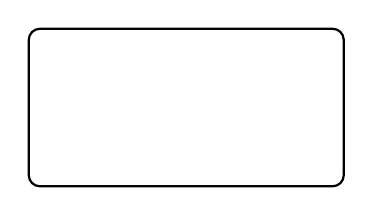
\begin{tikzpicture}
            \draw[thick, rounded corners] (0,0) rectangle (4,2);
        \end{tikzpicture}
    \end{minipage}

    \date{\today}
    \vfill
\end{titlepage}


\newpage % Ensure this file exists and is correctly formatted

% Table of contents
\newpage
{
  \setlength{\parskip}{0em}
  \renewcommand\contentsname{TABLE OF CONTENTS} % This will change heading text
  \tableofcontents \addcontentsline{toc}{section}{TABLE OF CONTENTS}
}

% List of figures - if any
\newpage
\listoffigures 
\addcontentsline{toc}{section}{LIST OF FIGURES}

% List of tables - if any
\newpage
\listoftables 
\addcontentsline{toc}{section}{LIST OF TABLES}
\pagenumbering{arabic}

\section{Background}
Cassava is a staple food crop grown in tropical and subtropical regions. It is valued for its high-yield tubers and nutrient-rich leaves. Its resilience in poor soils makes it a vital food source in many low-income regions. However, cassava plants are highly susceptible to several leaf diseases including Cassava Bacterial Blight (CBB), Cassava Brown Streak Disease (CBSD), Cassava Green Mottle (CGM), and Cassava Mosaic Disease (CMD). These diseases disrupt the photosynthetic process and significantly reduce crop yield and quality.

Conventional methods of disease detection involve laboratory testing or expert consultation, both of which are costly and time-consuming. As a result, farmers often lack the means to detect and treat diseases early. With recent advances in machine learning, especially in image classification using deep learning, it is now possible to build systems that can classify crop diseases from images with high accuracy and low cost. This project applies such techniques to develop a cassava leaf disease detection system.

\section{Problem Statement}
In regions like Bangladesh, where cassava is not yet widely cultivated but has strong potential, there is limited infrastructure for disease monitoring. Farmers lack tools for early and accurate identification of leaf diseases. Manual diagnosis is often not viable due to lack of expertise, cost, and time constraints.

This research focuses on the classification of cassava leaf diseases using machine learning models trained on labeled image datasets. The goal is to evaluate various deep learning models to determine which provides the best trade-off between accuracy and computational efficiency, ultimately aiding in timely and scalable disease detection.

\section{Chapter Distribution}
This report is organized into the following chapters:

\begin{itemize}
    \item \textbf{Chapter 1: Introduction} — Introduces the background of the study, identifies the research problem, and outlines the structure of the report.
    
    \item \textbf{Chapter 2: Literature Review} — Summarizes related works from at least eight research papers relevant to crop disease classification, focusing on methods, datasets, and performance metrics.

    \item \textbf{Chapter 3: Methodology} — Describes the overall method used in the project, details the machine learning models implemented, and explains the proposed framework that yielded the best performance.

    \item \textbf{Chapter 4: Experimental Result and Analysis} — Provides a description of the dataset, evaluation metrics, and parameter settings. It also discusses experimental results in detail, including error analysis, limitations, and the social or cultural impact of the proposed solution.

    \item \textbf{Chapter 5: Conclusion and Future Work} — Summarizes the research findings, reflects on the limitations, and suggests directions for future improvements and further study.
\end{itemize}

 % Ensure this file exists and is correctly formatted
\section{Problem Statement}
Currently, many travel agencies rely on outdated methods of booking and managing tour packages, often involving manual processes that can lead to inefficiencies, errors, and poor customer experience. Existing online systems may offer basic functionalities, but they frequently lack seamless integration between package selection, customization (e.g., flight and hotel preferences), and secure payment processing. Furthermore, the administrative management of packages and tour guide information is often cumbersome and not easily accessible.

This project aims to address these gaps by developing a user-friendly Travel Agency website that provides a fully integrated platform for browsing, selecting, and booking tour packages. The system will streamline the entire process, from browsing available options to customizing travel details and completing payment securely. Additionally, it will provide administrators with a robust interface to efficiently manage tour packages and local tour guide information. By addressing these challenges, this project will significantly improve the overall travel booking experience, making it more efficient for both customers and administrators.
\section{Objectives}

\begin{enumerate}
    \item \textbf{Develop a User-Friendly Interface}  
    \begin{itemize}
        \item \textbf{Specific}: Create an intuitive and responsive website interface that allows users to browse and select tour packages, choose flight and hotel types, and proceed to a payment gateway.  
        \item \textbf{Measurable}: Ensure the website is fully functional on desktop and mobile devices with at least 90\% user satisfaction in usability tests.  
        \item \textbf{Achievable}: Leverage modern web development technologies such as Node.js, Next.js, and Tailwind CSS to build the interface.  
        \item \textbf{Relevant}: This objective addresses the need for a seamless and convenient user experience.  
        \item \textbf{Time-bound}: Complete within the first 2 months of the project timeline.
    \end{itemize}

    \item \textbf{Implement Secure Payment Gateway Integration}  
    \begin{itemize}
        \item \textbf{Specific}: Integrate a reliable and secure payment gateway to handle user transactions when booking tour packages.  
        \item \textbf{Measurable}: Successfully complete payment transactions in at least 95\% of test cases with no security vulnerabilities.  
        \item \textbf{Achievable}: Use trusted APIs and payment systems such as Stripe or PayPal for integration.  
        \item \textbf{Relevant}: This ensures that users can make secure payments, directly addressing the issue of manual payment handling.  
        \item \textbf{Time-bound}: Implement within 3 months of the project timeline.
    \end{itemize}

    \item \textbf{Develop Admin Panel for Package and Guide Management}  
    \begin{itemize}
        \item \textbf{Specific}: Build an admin interface that allows easy CRUD operations on tour packages and the addition of local tour guide information.  
        \item \textbf{Measurable}: Ensure the admin panel has full functionality for managing at least 50 tour packages and guide details.  
        \item \textbf{Achievable}: Use MySQL for database management and integrate with the website’s backend system.  
        \item \textbf{Relevant}: This directly addresses the inefficiencies in current systems for package and guide management.  
        \item \textbf{Time-bound}: Complete the admin panel within 4 months.
    \end{itemize}

    \item \textbf{Ensure System Scalability and Performance Optimization}  
    \begin{itemize}
        \item \textbf{Specific}: Optimize the website's backend for performance, ensuring that it can handle a large volume of concurrent users and data.  
        \item \textbf{Measurable}: Achieve load times under 2 seconds and handle up to 500 simultaneous users in stress tests.  
        \item \textbf{Achievable}: Utilize best practices for web performance and use efficient database queries and caching mechanisms.  
        \item \textbf{Relevant}: Ensuring scalability will allow the system to accommodate growth and handle peak traffic periods.  
        \item \textbf{Time-bound}: Complete optimization within the final month of the project.
    \end{itemize}

    \item \textbf{Conduct User Testing and Feedback Collection}  
    \begin{itemize}
        \item \textbf{Specific}: Perform user testing with at least 30 participants to gather feedback on usability, design, and functionality.  
        \item \textbf{Measurable}: Collect and analyze feedback with a goal of improving the system based on at least 80\% of the user suggestions.  
        \item \textbf{Achievable}: Organize user testing sessions through surveys and usability tests.  
        \item \textbf{Relevant}: This will ensure that the platform meets user expectations and functions as intended.  
        \item \textbf{Time-bound}: Conduct testing during the last 2 weeks of the project.
    \end{itemize}
\end{enumerate}

By achieving these objectives, the project will significantly improve the travel booking process, ensuring ease of use for customers and efficiency for administrators.

\newpage
\section{Methodology}
This section outlines the systematic approach followed during the development of the travel agency website. The Software Development Life Cycle (SDLC) model was followed to ensure that the project was well-organized, efficient, and delivered successfully within the given timeframe.

\subsection{Planning}
The planning phase involved identifying project goals, features, and tools. The stack was finalized to include HTML, Tailwind CSS, JavaScript, and Next.js for the frontend, and Laravel with MySQL for the backend. Requirements were gathered for both the user and admin roles, and the expected user journey was mapped out—from viewing packages to payment completion.

\subsection{Design}
The design phase included both frontend and backend architectural planning. Wireframes were drawn to visualize page layouts such as Home, Package Listing, and Booking pages. The backend was structured using Laravel's MVC architecture. ER diagrams were created to model database relationships for users, packages, bookings, and tour guides.

\subsection{Implementation}
Frontend pages were built using Next.js for server-side rendering and faster load times. Tailwind CSS was used for consistent, responsive styling. On the backend, Laravel handled routing, controllers, models, and database migrations. Admin features like CRUD operations for tour packages and guide management were also implemented here.

\subsection{Testing}
Unit and integration testing were carried out to ensure all features worked as intended. Laravel’s built-in testing tools were used to test backend logic. Frontend behavior was manually tested across different browsers and devices. Form validation and session handling were thoroughly checked.

\subsection{Deployment}
After successful testing, the application was prepared for deployment. The backend (Laravel) was hosted on a PHP-compatible server, and the Next.js frontend was deployed via Vercel or a Node-compatible server. Environment variables were configured for secure communication with the database and third-party services.

\subsection{Future Enhancements}
Possible future improvements include integrating a real-time chatbot for customer support, adding review and rating features for packages, incorporating real-time availability for flights and hotels via APIs, and building a mobile app version of the platform using React Native.

\newpage
\section{Expected Output}
Describe the anticipated results of the project. Explain how these outcomes will address the problem statement and meet the objectives. Discuss the potential impact or benefits of the project, including any contributions to knowledge or practical applications.

Describe the expected outcomes and deliverables of your project. Explain how the successful completion of your project will contribute to solving the problem and achieving the stated objectives. Discuss the potential benefits, impacts, or implications of your project.

% References
\phantomsection
\addcontentsline{toc}{section}{REFERENCES}  % Add to Table of Contents

% Citing references
% Add references to bibliography, but do not cite in text
\nocite{ref1, ref2, ref3, ref4, ref5, ref6, ref7}


\bibliographystyle{IEEEtran}  % Choose your bibliography style

\bibliography{biblio}  % Make sure 'biblio' matches the name of your .bib file (without the .bib extension)

\end{document}